\documentclass[11pt, fleqn]{article}

\usepackage[usenames,dvipsnames,svgnames,table]{xcolor}
\usepackage{amsmath}
\usepackage{amsfonts}
\usepackage[margin=1in]{geometry} % To set the margin widths
\usepackage{graphicx}
\usepackage{listings}
\usepackage{multirow}
\usepackage{tabularx}
\usepackage{varioref}
\usepackage[noabbrev,capitalize]{cleveref}
\usepackage[group-separator={,}]{siunitx}
\usepackage{subcaption}
\usepackage{titlesec}
\usepackage{lscape}
\usepackage{bm}
\usepackage{chngpage}
\usepackage[titletoc,toc,title]{appendix}

\renewcommand\thesection{\arabic{section}}
\renewcommand\thesubsection{\thesection\alph{subsection}}

\lstset{
  frame=single,
  basicstyle=\ttfamily,% print whole listing small
  language=R,
  aboveskip=3mm,
  belowskip=3mm,
  showstringspaces=false,
  columns=flexible,
  numbers=none,
  commentstyle=\color{ForestGreen},
  stringstyle=\color{Maroon},
  breaklines=true,
  breakatwhitespace=true,
  tabsize=2,
  literate={<-}{{$\gets$}}1 {~}{{$\sim$}}1
}

\sisetup{output-exponent-marker=\textsc{e}}

\setlength{\parskip}{12pt} % Sets a blank line in between paragraphs
\setlength\parindent{0pt} % Sets the indent for each paragraph to zero

\begin{document}

\title{Homework \#3\\
Digital and Algorithmic Marketing (37304-01)}
\author{
Brian Chingono, Will Clark, Matthew DeLio, Jonathan Stevens (\textbf{Group \#8})\\
University of Chicago Booth School of Business}

\maketitle

\section{Gender-Based Preferences of Message Senders}

\cref{fig:heatmap_female} and \cref{fig:heatmap_male} show, for a given sender rating, the difference between the conditional probability of sending a message (conditioned on the senders rating) and the marginal probability of sending a message across all receiver ratings.

\begin{figure}[!htb]
  \centering
  \caption{}
  \begin{subfigure}[b]{0.49\textwidth}
    \caption{Relative Preferences of Female Senders}
    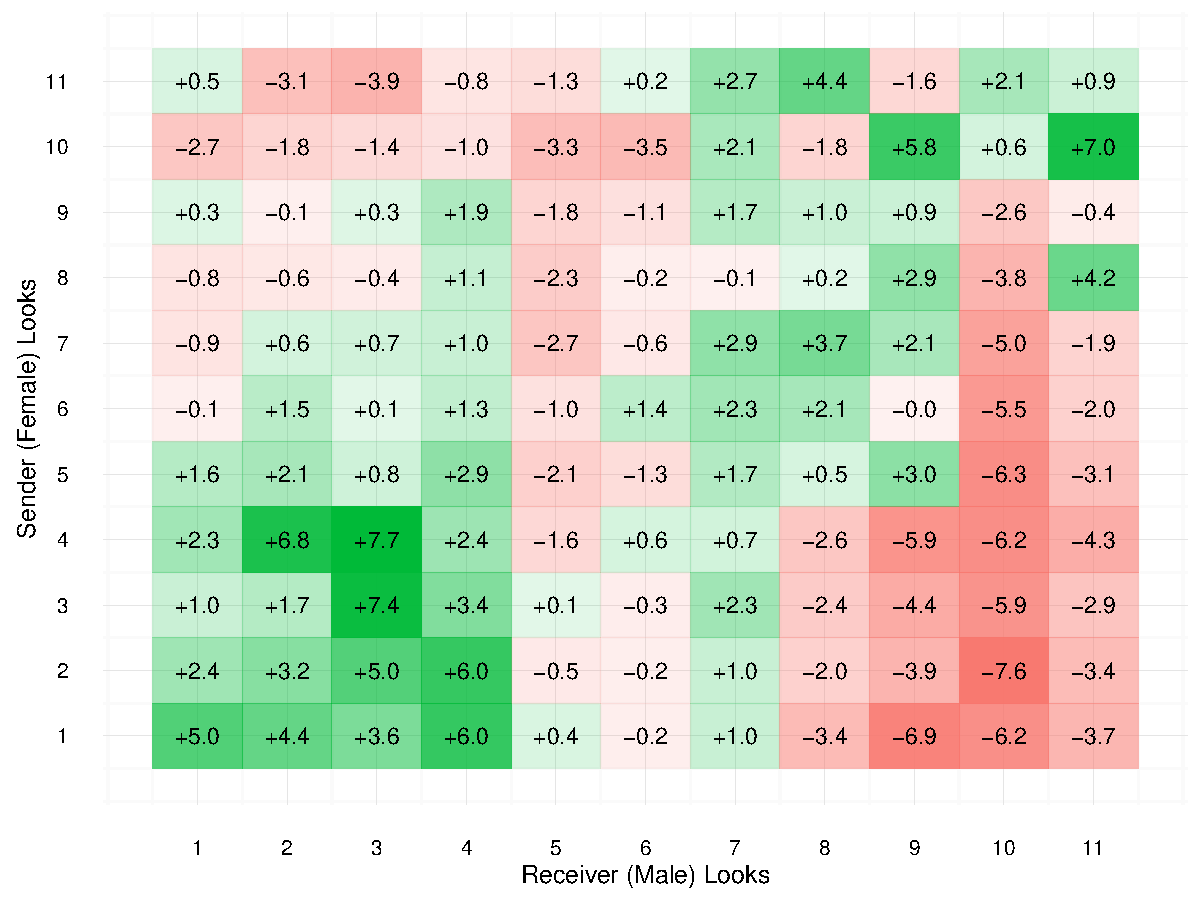
\includegraphics[width=\textwidth]{heatmap_female.pdf}
    \label{fig:heatmap_female}
  \end{subfigure}
  \hfill
  \begin{subfigure}[b]{0.49\textwidth}
    \caption{Relative Preferences of Male Senders}
    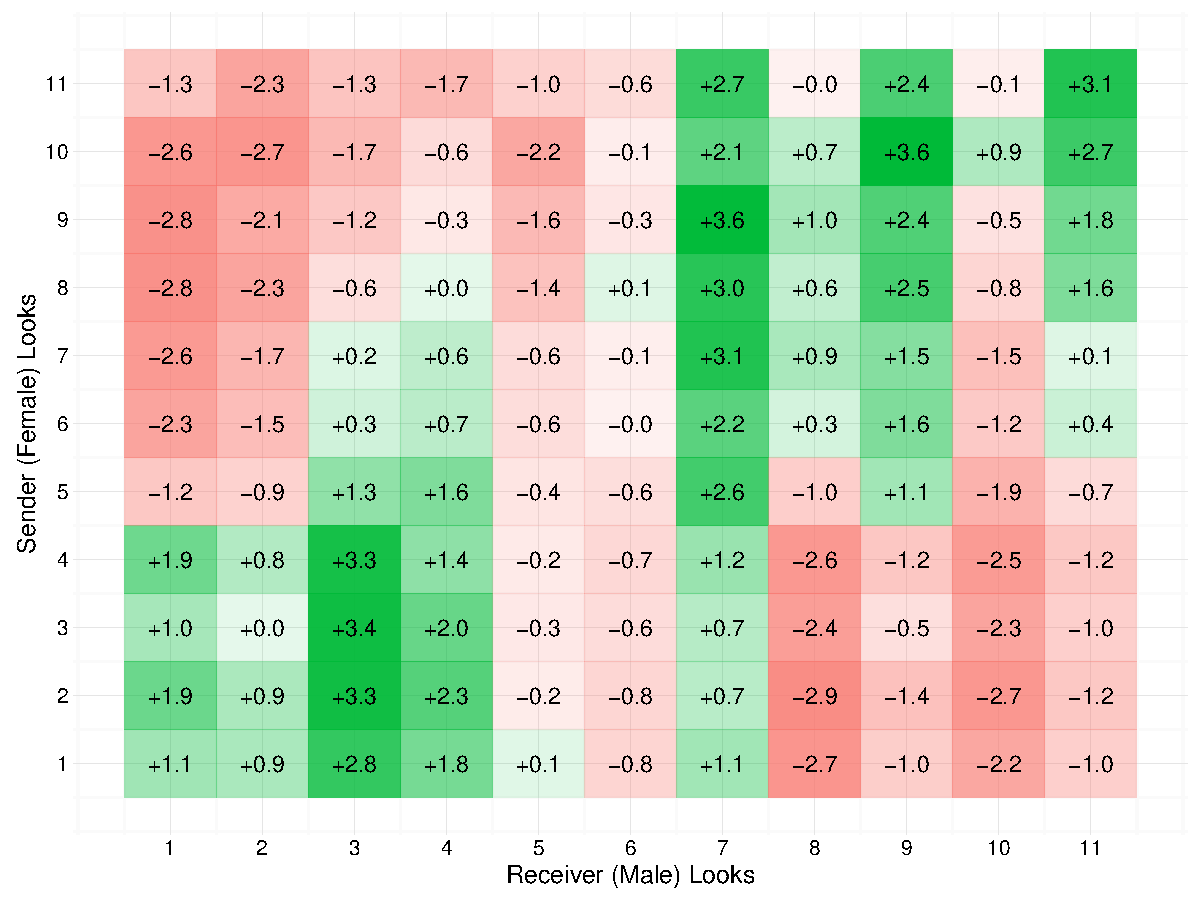
\includegraphics[width=\textwidth]{heatmap_male.pdf}
    \label{fig:heatmap_male}
  \end{subfigure}
\end{figure}

\begin{figure}[!htb]
  \centering
  \caption{}
  \begin{subfigure}[b]{0.49\textwidth}
    \caption{Aggregate Sending Behavior of Females}
    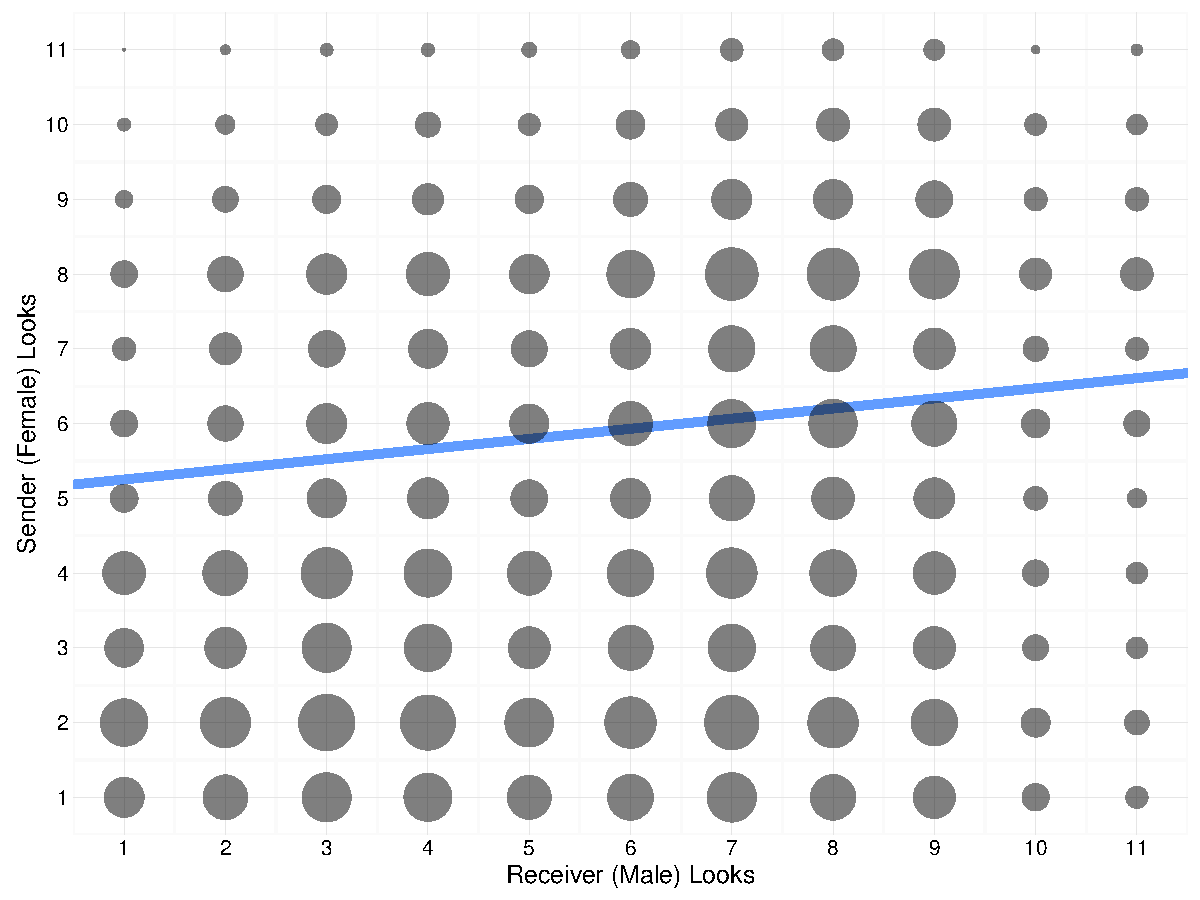
\includegraphics[width=\textwidth]{dotplot_female.pdf}
    \label{fig:dotplot_female}
  \end{subfigure}
  \hfill
  \begin{subfigure}[b]{0.49\textwidth}
    \caption{Aggregate Sending Behavior of Males}
    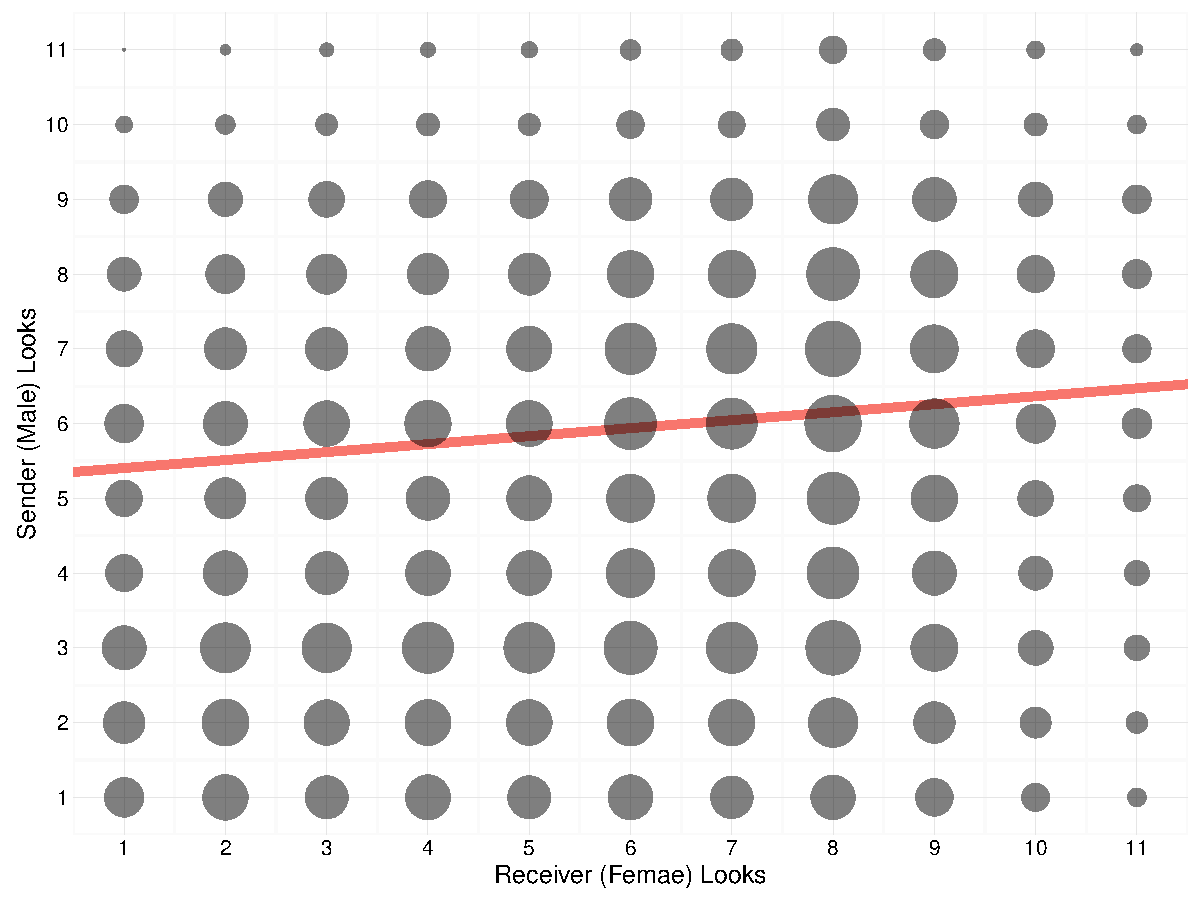
\includegraphics[width=\textwidth]{dotplot_male.pdf}
    \label{fig:dotplot_male}
  \end{subfigure}
\end{figure}

%%%%%%%%%%% BEGIN APPENDIX
\clearpage
\section{Appendix} \label{sec:appendix}

\end{document}

% \input{.tex}

% \begin{figure}[!htb]
%   \centering
%   \caption{}
%   \begin{subfigure}[b]{0.49\textwidth}
%     \caption{}
%     \includegraphics[width=\textwidth]{.pdf}
%     \label{fig:}
%   \end{subfigure}
%   \hfill
%   \begin{subfigure}[b]{0.49\textwidth}
%     \caption{}
%     \includegraphics[width=\textwidth]{.pdf}
%     \label{fig:}
%   \end{subfigure}
% \end{figure}

% \begin{figure}[!htb]
%   \centering
%   \caption{}
%   \includegraphics[scale=.5]{.pdf}
%   \label{fig:}
% \end{figure}